\documentclass{article}
\usepackage[utf8]{inputenc}
\usepackage{todonotes}
\usepackage{array}
\usepackage{subcaption}
\usepackage{graphicx}
\usepackage{wrapfig}
\usepackage{float}

\title{CSC470: Software Engineering Final Report\\ TESS: The Extraordinary Sudoku Solver}
\author{Team: \#1 \\David Koval and Joseph Mammo\\Instructor: Dr. Ahyoung Lee}
\date{ 4/24/17 \\ v1.1 }

 
\renewcommand*\contentsname{Table of Contents}

 
\begin{document}
 
\maketitle

\clearpage

\tableofcontents

\clearpage

\section{Executive Summary} 

Have you ever played a Sudoku game that you weren’t able to solve? Have you spent hours trying to solve a specific puzzle, but something never quite added up? This is where The Extraordinary Sudoku Solver (TESS) comes in; an Android application developed by David Koval and Joseph Mammo, TESS isn’t just a normal sudoku game: it allows normal game play and has an added feature that makes it stand out from the rest of the Android apps currently on the Play Store – solving any given Sudoku puzzles***. \newline \newline
The goal of TESS is to allow a user to play different sudoku games, much like most of the apps currently out there, but also allow a user to input a sudoku puzzle they have been working on elsewhere and get an instant solution. TESS allows the user to select difficulty level, ranging from 1 – 5 (easy to hard), and play a regular 9x9 sudoku game in an intuitive interface. By utilizing a depth search with pruning algorithm, our game solves most Sudoku puzzles in under 5 seconds. Furthermore, TESS lets the user check their boards and highlights any invalid inputs.\newline \newline
With a black and neon green coloring design, TESS simulates a hacker experience; and with its intuitive button design, TESS makes it tremendously easy to choose, play and/or solve sudoku games with any difficulty levels. The user can select play or solve at the very beginning. If the user decides to play a game, then they will be able to choose a difficulty they would like to play. During game play. The user is provided with a hint button (currently under development) to get hint to solve the puzzle; a check button to check status of their board; a solve button to solve the rest of the puzzle; delete and clear buttons to remove a single value and remove all values on the board respectively; the user can select the quit option to exit the current board and return to the main menu. After the quit sequence is initiated, TESS saves the current progress of the user in a database so the user can resume at any time. The following description is outlined in Figure \ref{fig:current}. The sequence diagram (Figure \ref{fig:sequencediagram}) illustrates the flow of logic when a user decides to play the game. Finally, the activity diagram (Figure \ref{fig:activitydiagram}) greatly outlines the dynamic aspects of the proposed sudoku game.  \newline \newline
The test plan for this project is based on the bottom-up approach. We, the developers, focused on utility, reliability, robustness, and performance to ensure this project is functional and well as enjoyable to the user. We performed 1 White-box test where each method is directly dependent on the other to produce the correct solution and 1 other White-box test to perform the same test on invalid input. Due to the nature of the project, the integration testing is directly associated with the unit testing. \newline \newline
To sum up, TESS allows a user to play and solve a regular 9x9 sudoku game. The game provides level based Sudoku games and saves the progress of the puzzle upon quitting so the user can resume their game. Because of its intuitive design, solving functionality and all-inclusive bottom up testing approach, TESS stands out from most Sudoku apps that are currently published on the Google Play Store. \newline \newline
As a future work, we plan to add more challenging puzzles based on different difficulty levels; improve the current solving feature by implementing the paper-and-pen algorithm; and open-source the project so anyone can adapt our code and add more features to TESS. 

 
\section{Introduction}
This documentation is in support of The Extraordinary Sudoku Solver (TESS) application implemented in Android Studio using Java programming language on a Windows operating system. The document assumes that the reader is already familiar with using Android Studio programming in Java. \newline \newline
The intent of this documentation is to provide an in-depth explanation of the requirement specifications, system design, implementation and testing of TESS. \todo{ [More info]} \newline \newline
The documentation starts with stating the purpose of the documentation and outlining the definitions, acronyms and abbreviations used in the documentation. In the third section, the documentation states the goals of TESS followed by the functional and non-functional requirements of the Android application. Then the documentation unpacks the system model of TESS through a use case diagram and a traceability matrix. Finally, system design and implementation are presented at the last two sections of this document. 

\subsection{Purpose}
The purpose of this document is to give a detailed and overall description of The Extraordinary Sudoku Solver (TESS) app. The overall purpose of this project is to help the avid Sudoku players to have a platform to enjoy the game on as well as get help when they are unable to solve a puzzle. This app is intended to be used by both amateurs and professionals, as well as anyone in-between. This will be a free platform for anyone to have access to it as well as modify it in any way the like. Sudoku is an amazing game and the hopes of this project is to expand the entertainment and excitement of Sudoku to anyone willing to try this app.

\subsection{Definitions, acronyms, and abbreviations}

\begin{tabular}{ | m{8em} | m{24em}|  } 
\hline
\textbf{Term}& \textbf{Definition}  \\ 
\hline
DESC & Description  \\ 
\hline
DFS & Depth First Search Algorithm\\
\hline
Grid & This is where all the values are stored for the player to see.  \\ 
\hline
ID & Identification  \\ 
\hline
PW & Priority Weights  \\ 
\hline
User & Whoever will be using the app  \\ 
\hline
\end{tabular}

 

\section{Goals}
There are a few major goals that needed to be accomplished in this project. The main overaching goal was to create an intuitive Sudoku game UI and combine it with a Sudoku game solving component. This goal was thus broken into smaller pieces: create a user friendly UI for a user to be able to play a Sudoku game and create a efficient and fast Sudoku solver to solve any given puzzle. This program also needed to have a few additional components as well. The program must include some sort of searching algorithm and because of the complexity of the problem, it also needs to include some sort of pruning technique to minimize the operations needed to solve the entire game. The program also have some sort of database component to store all the puzzles in along with the current puzzle the user is working on. Another major goal was to turn this program into a mobile app that will run on Android devices and eventually on other systems as well. These were the main goals of the project that helped drive the focus of the project and its workers.

 
\section{Specific Requirements}
This section will cover the specific requirements of the project including functional and non-functional requirements. The functional requirements are identified with R followed by a number and nonfunctional requirements are identified with RQ followed by a number. All the functional requirements are marked with a PW (Priority Weight) which refer to the priority of that specific requirement with 5 being the highest priority and 1 being the lowest.

 
\subsection{Functional Requirements}
This section will cover the functional requirements associated with the project along with the following tags: ID, TITLE, DESC, and PW. \newline \newline
\textbf{ID:R1} \newline TITLE: Play Game Option\newline DESC: The user first opens up the app, they should be able to choose the option to play a Sudoku puzzle. They user should be able to stay as long as they want to on this screen.\newline PW: 3 \newline \newline
\textbf{ID:R2} \newline TITLE: Select Difficulty \newline DESC: The user should be able to select a difficulty setting that better suites needs at any time. There should be 5 difficulty options for the user to choose from. 1 being the easiest all the way down to 5 being the hardest.\newline PW: 2 \newline \newline
\textbf{ID:R3} \newline TITLE: Back Option \newline DESC: The user should be able to return to the main screen from the select difficulty screen if they don't select a difficulty. The user can remain on the select difficulty as long as the want to.\newline PW: 1 \newline \newline
\textbf{ID:R4} \newline TITLE: Continue Game \newline DESC: The user should be able to continue a game that has been previously started whether or not the app has been closed. All of the user's input should be saved so they could be brought up again should the user want to continue a game.\newline PW: 4 \newline \newline
\textbf{ID:R5} \newline TITLE: Get Puzzle \newline DESC: When the user selects a difficulty, a puzzle with the selected difficulty should be retrieved from the database for the user to be able to play it and enjoy the game.\newline PW: 2 \newline \newline
\textbf{ID:R6} \newline TITLE: Solver Option \newline DESC: On started, the user should be able to select the Solver option in the app to go straight to the solver part of the app. \newline PW: 5 \newline \newline
\textbf{ID:R7} \newline TITLE: Input Sudoku Puzzle To Solve \newline DESC: The user needs to be able to input any sort of Sudoku puzzle that the user has, with or without any extra numbers the user wishes to input. \newline PW: 5 \newline \newline
\textbf{ID:R8} \newline TITLE: Check Current Board \newline DESC: The user should be able to check the status of the current puzzle they are working on. The user should be able to view the inputs that are conflicting with each other. They should be marked in some way for the user to be able to see them clearly. \newline PW: 4 \newline \newline
\textbf{ID:R9} \newline TITLE: Delete an Input Value \newline DESC: The user should be able to delete an input value that they put in previously or a value that the system put in automatically. \newline PW: 5 \newline \newline
\textbf{ID:R10} \newline TITLE: Clear Board \newline DESC: The user should be able to clear the entire board easily and effortlessly. \newline PW: 3 \newline \newline
\textbf{ID:R11} \newline TITLE: Solve Current Board \newline DESC: The user should be able to have the option to solve the current board that they are working on. It should use the input the system put in as well as the inputs the user decided to add. \newline PW: 5 \newline \newline
\textbf{ID:R12} \newline TITLE: Play Sudoku Game \newline DESC: The user should be able to play a Sudoku game by selecting certain boxes and input a value into them. \newline PW: 4 \newline \newline
\textbf{ID:R13} \newline TITLE: Hint Option \newline DESC: The user should have the option to get a hint on the current Sudoku game they are playing. The hint should display any correct value on the given board. \newline PW: 1 \newline \newline
\textbf{ID:R14} \newline TITLE: Download Mobile Application \newline DESC: The user should be able to download the mobile application either from the Play Store or via Email to their Android phone. The download should be free. \newline PW: 5 \newline 

\subsection{Non-Functional Requirements} 
This section will cover the non-functional requirements associated with the project along with the following tags: ID, TITLE, and DESC. \newline \newline
\textbf{ID:RQ1} \newline TITLE: System Availability \newline DESC: The system needs to  be available to the user 99.9\% of the time, whether or not the system is being used. The system can only be down for 0.1\% of the time for updates or maintenance. \newline \newline
\textbf{ID:RQ2} \newline TITLE: Solve Time \newline DESC: The app should be able to solve a given Sudoku puzzle, whether there is or isn't a solution in under 5 seconds.\newline \newline
\textbf{ID:RQ3} \newline TITLE: Search Algorithm \newline DESC: The Suduko solver must utilize some search algorithm such as depth first search or breadth first search or any other searching algorithm. \newline \newline
\textbf{ID:RQ4} \newline TITLE: Pruning Technique \newline DESC: There must be some sort of pruning technique with solving the problem because 9\textsuperscript{81} is not feasible. \newline \newline
\textbf{ID:RQ5} \newline TITLE: Database Storage \newline DESC: The Database needs be stored locally on the device and new puzzles should be added to the device through updates or pulled from an external database. \newline \newline
\textbf{ID:RQ6} \newline TITLE: Easy to Use \newline DESC: The app should be very simple to use to any player with some general idea of how Sudoku puzzles work. \newline \newline
\textbf{ID:RQ7} \newline TITLE: Private Information \newline DESC: The app should not keep any personal information about the user. There app should not ask the user for any passwords. \newline \newline

\subsection{Version}
This is version 1.1 or v1.1, which is also the most current version of the system. Version 1.0 came out on the April 7, 2017; however, after tests were conducted there were a few design flaws that needed to be worked around. Version 1.0 was not able to solve difficult Sudoku puzzles within the allotted and many of the beta testers were not pleased with this. After some thought, v1.0 was pulled off the market and developers continued to improve the algorithm to solve the more difficult problems. In v1.1, the developers finally came up with a fast enough algorithm to solve it within the time limit. This new and updated version will be available on the market soon; however, it still remains in its early stages of development. 

\subsection{System Model}
This section will cover the general system model. This section includes the actors, use cases, use case diagram, prototyping and the traceability matrix.
\subsubsection{Actors}
The section covers the primary actors that are involved with the system directly or indirectly. \newline
\begin{itemize}
   \item Player: This is the primary actor who will be using the app as well as interacting with it.
   \item Database: This is the datastore that is on the device that contains all the Sudoku puzzles for the user to play.
\end{itemize}

\subsubsection{Use Cases}
This section covers the use cases that are most prominant in the Sudoku app that describe how the user shall interact with the app. Each use case will contain the following components: ID, Title, Actors, and Description.\newline \newline
\textbf{ID:UC1} \newline TITLE: Select Play Game \newline ACTORS: Player \newline DESC: Player opens up the app and selects to play a Sudoku puzzle. \newline \newline
\textbf{ID:UC2} \newline TITLE: Select Solver \newline ACTORS: Player \newline DESC: Player opens up the app and selects the Solver option to solve a Sudoku puzzle they might have. \newline \newline
\textbf{ID:UC3} \newline TITLE: Selecting a difficulty \newline ACTORS: Player and Database\newline DESC: Player selects a difficulty from the options available and a Sudoku board is filled with a puzzle similar to the difficulty the Player selected. \newline \newline
\textbf{ID:UC4} \newline TITLE: Quitting Time \newline ACTORS: Player and Database \newline DESC: When Player decides to quit the puzzle they are currently working on, the puzzle is saved to the database so Player can continue playing it.  \newline \newline
\textbf{ID:UC5} \newline TITLE: Continuing \newline ACTORS: Player and Database \newline DESC: When Player decides to play a game again and selects the continue option to bring up the previously saved game they were playing. \newline \newline
\textbf{ID:UC6} \newline TITLE: Give me a hint \newline ACTORS: Player \newline DESC: The Player is unsure of any other moves, so Player decides to select the hint option in order to recieve a hint about the current Sudoku puzzle they are working on. \newline \newline
\textbf{ID:UC7} \newline TITLE: Solve the Puzzle \newline ACTORS: Player \newline DESC: The Player is tired of playing and wants to see the solution to the Sudoku puzzle, so they decided to tap the solve button to get all the answers. \newline \newline
\textbf{ID:UC8} \newline TITLE: Clear the Board \newline ACTORS: Player \newline DESC: The Player decides to start a new puzzle, so the Player hits the clear button to erase everything on the board. \newline \newline
\textbf{ID:UC9} \newline TITLE: Playing the game \newline ACTORS: Player \newline DESC: The Player enjoys playing a Sudoku game by clicking the buttons and entering the numbers that they might think will solve the puzzle. \newline

\subsubsection{Use Case Diagram}
Figure \ref{fig:usecasediagram} depicts the the use case diagram used by the app as well as the develops to design a proper system. The diagram shows the interaction between the different users as well the correlation it has with the different use cases.
\begin{figure*}[h!]\centering
	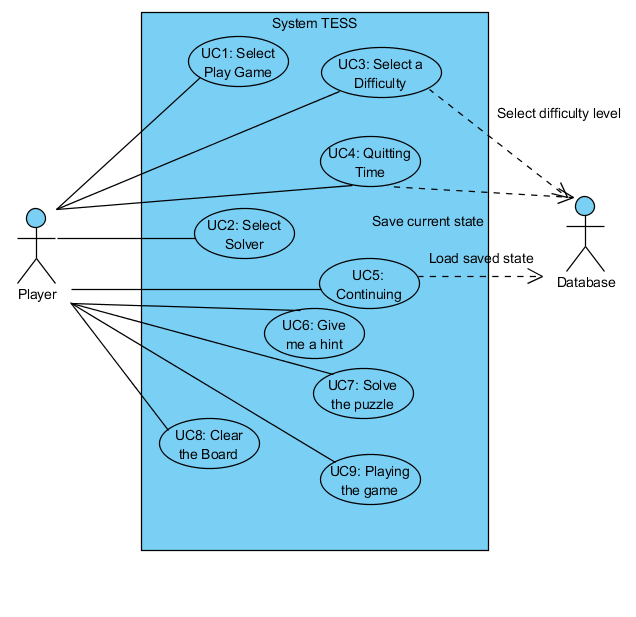
\includegraphics[width=4.0in]{./Figure/Usecase_Diagram.PNG}
	\caption{Use case diagram of the TESS System.}\label{fig:usecasediagram}
\end{figure*}

\subsubsection{Traceability Matrix}
The traceability matrix, as shown in Figure \ref{fig:traceabilitymatrix}, shows the priority weight of each use case based on the requirements that it meets. As per the figure, use case 9 had one of the highest priorities, which is consequently one of the most important use cases as well. The diagram shows the different use cases and how the corrolate with the different requirements. It also helps depict which use cases are the most important based off the priority weights.
\begin{figure*}[h!]\centering
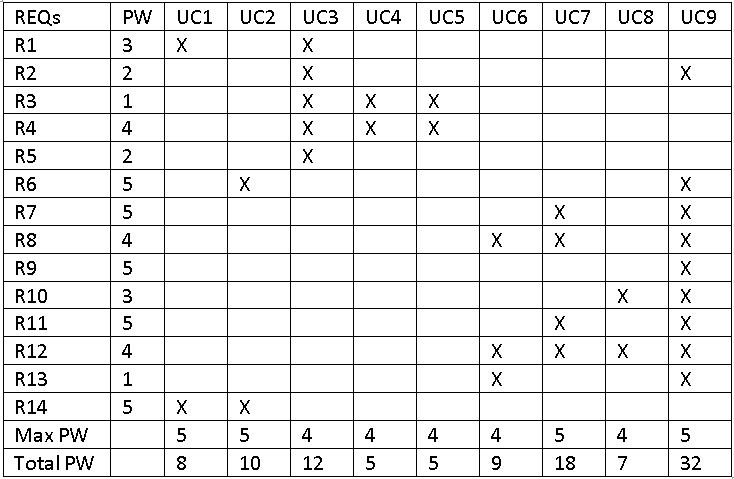
\includegraphics[width=4.0in]{./Figure/Traceability_Matrix.PNG}
\caption{Traceability Matrix of the TESS System.}\label{fig:traceabilitymatrix}
\end{figure*}

\section{System Design}
This section will cover the overall design of the TESS system along with constaints and alternative designs to the system.

\subsection{Design Overview}
This section will provide the the design overview of the TESS system. The system resemblance had to be close to what the game looks like in real life. So the developers had an idea with what they would be creating. Soon after the client game the developers a hand drawn image, Figure \ref{fig:initialDesign}, to help the developers out.

\begin{figure}[h]
\centering
\begin{minipage}{.5\textwidth} \centering 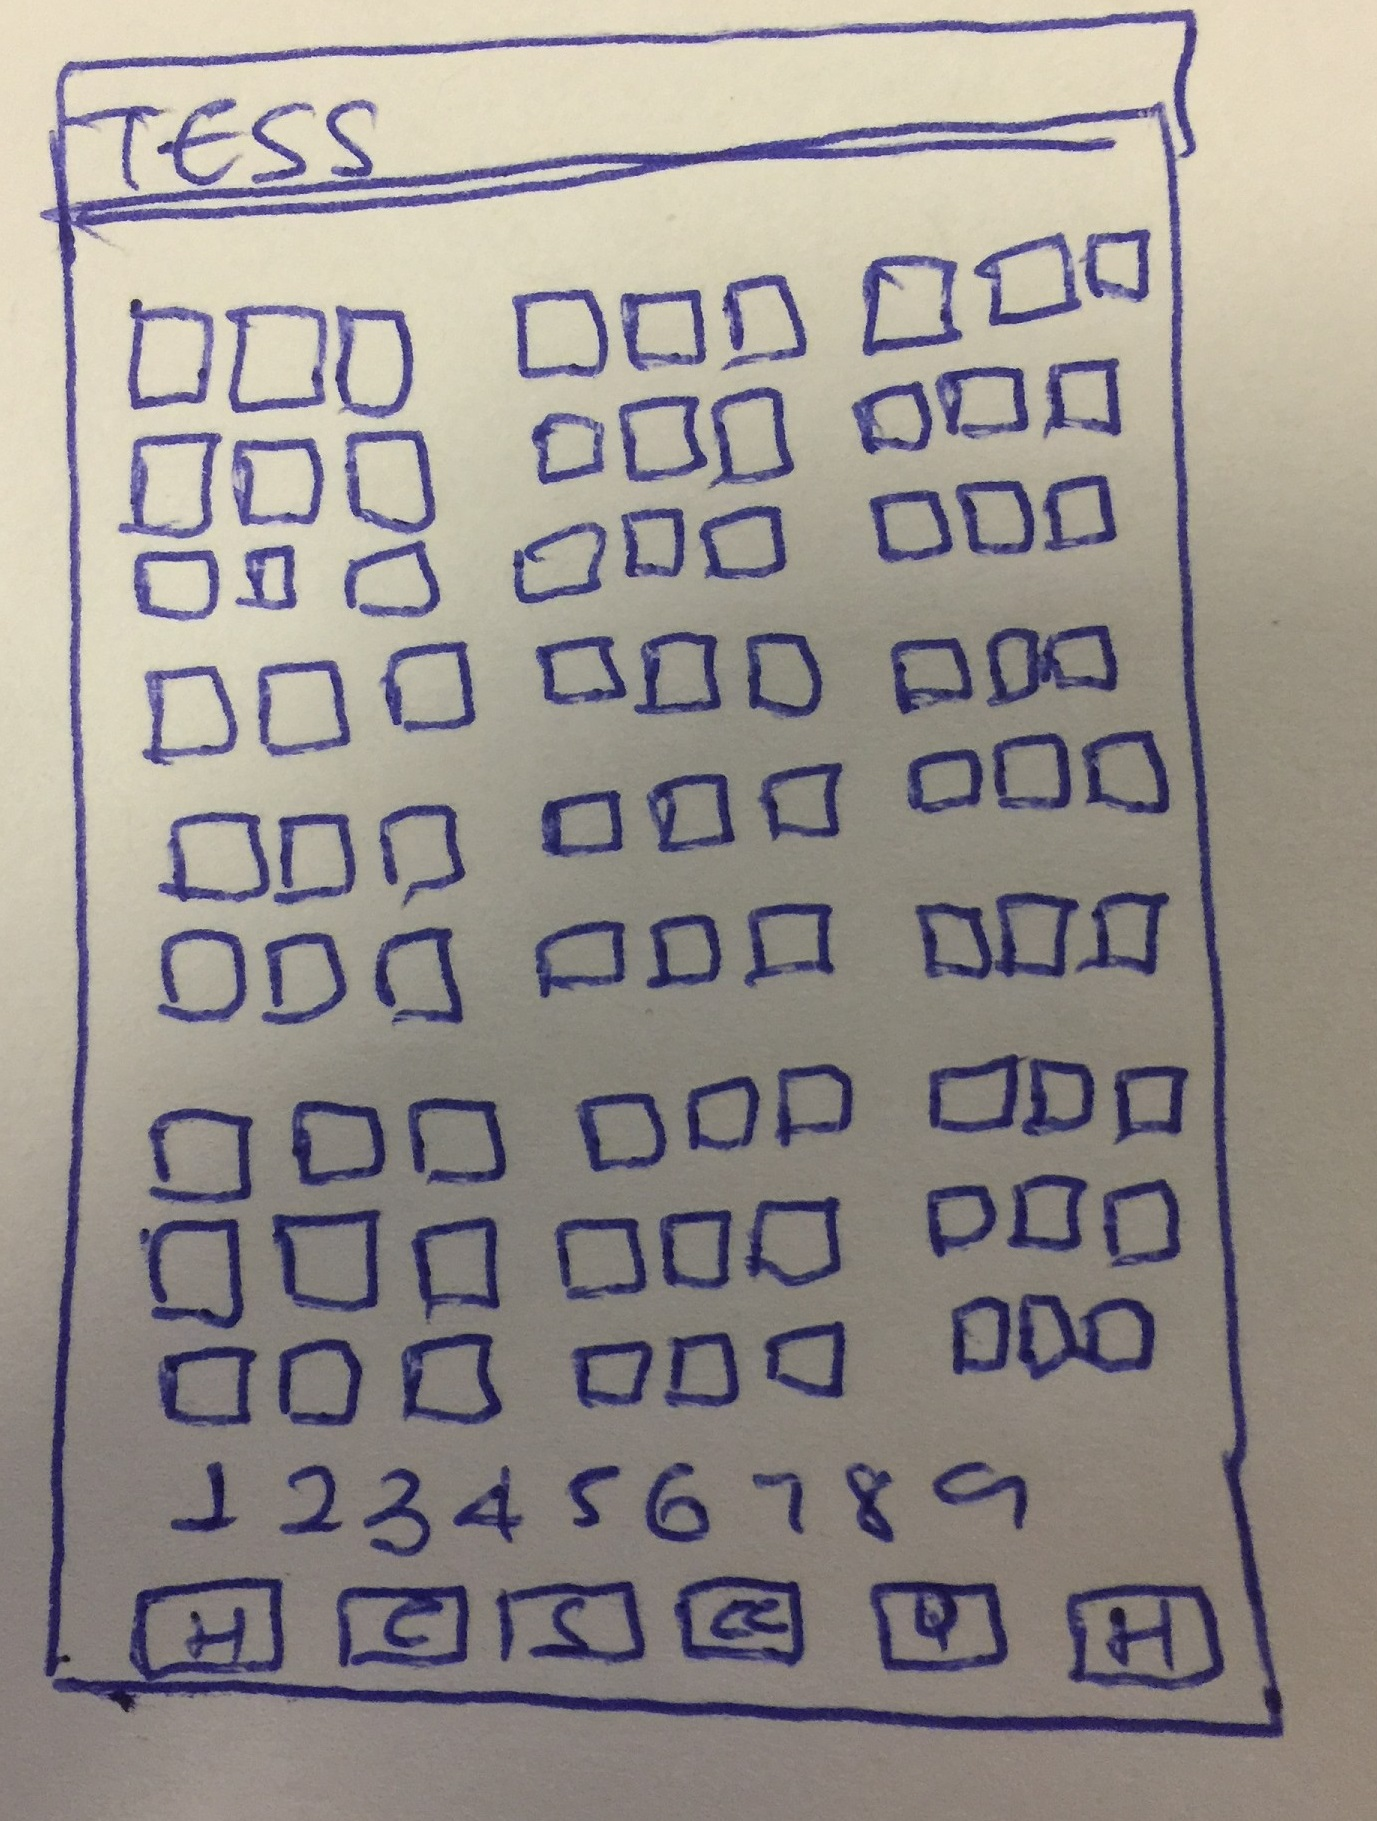
\includegraphics[width=2in]{./Figure/initial_design.jpg}\captionof{figure}{Initial Design of TESS System} \label{fig:initialDesign}
\end{minipage}%
\begin{minipage}{.5\textwidth}\centering 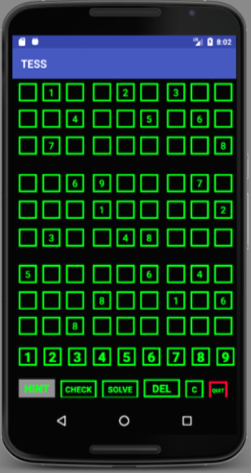
\includegraphics[width=2.0in]{./Figure/currentBoard.PNG} \captionof{figure}{Current Design of TESS System}\label{fig:current}
\end{minipage}%
\end{figure}
\begin{figure*}[h]
	\centering
	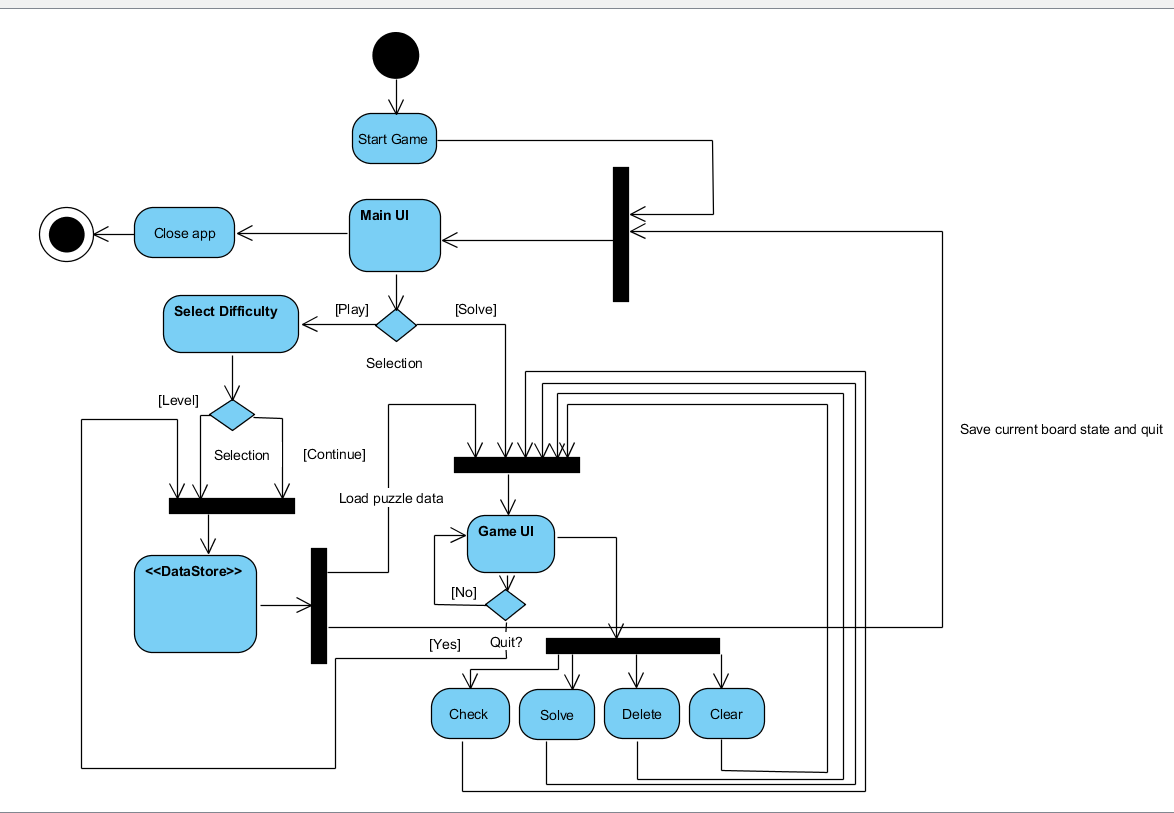
\includegraphics[width=5in]{./Figure/Activity_Diagram.PNG}
	\caption{Activity diagram of the TESS system.}\label{fig:activitydiagram}
\end{figure*}
The initial design was a simple 9x9 board with a set of numbers near the bottom of the screen numbered 1 through 9. There were also a few buttons underneath those that resembled extra options; they were: quit, solve, hint, clear, delete, and check. At first the developers where unsure what those meant; however, the client soon clarified those up. The quit button was a command to quit the game, but there was also a hidden feature to that option. When the user would quit, that button would save the current board into the database to save the current state. After much careful planning the deveopers were able to come up with a board similar to the one drawn as depicted in Figure \ref{fig:current}. The client had approved the design so the developers continued to work on the backend work based on the requirements. To make the development easier an activity diagram, as shown in Figure \ref{fig:activitydiagram}, was created to show the workflow of events. The diagrams shows the start node, which leads to the main UI page. From the main UI page the user could select either the play option or the solve option. If the solve option is selected, it goes to a select difficulty page and allows the user to select a difficulty. From there the user can either continue a puzzle or select a difficulty they would like to play. The puzzle is then loaded. The solver option would eventually lead to the same page as the other option, but the board would be clean. The diagram helps show the different options and well the possible routes a user could take while playing the game. From that diagram, it is visible that there need to be at least 3 main UI pages as well as some of the capabilities such as solve and hint. With the help of these diagrams depicting the flow of data, the developers were able to come up with a sophisticated design of TESS.

\subsection{System Constraints and Professional Standards}

First, the game should follow the rules outlined for a regular 9x9 sudoku game. Second, the application needs to solve a given puzzle in a timely manner. Third, the game must implement a database system to save and retrieve sudoku puzzles. Fourth, the game must not take more than 5MBs of memory and have access to an Internet connection for future updates. Lastly, the application must be designed to work for devices running the Android operating system. \newline \newline
The application design for Android smartphones requires to be implemented in Java. In addition to the programming language requirements, Android application development requires Android Studio integrated development environment (IDE) to be installed on the development computer. The IDE enables the developer to program and test the app on the same computer.\newline \newline
The IDE itself requires the developer to have a basic understanding of Android application development. It also requires the developer to configure an Android Virtual Device to run and test the app that is currently being developed. 
\newline \newline
We have outlined the seven system constraints of TESS below. 
\newline \newline
\textbf{ID:C1} \newline TITLE: Memory Space \newline DESC: The app should have a small footprint. The entire app should take up less than 5MBs of memory, this is including with future updates as well.\newline\newline
\textbf{ID:C2} \newline TITLE: Internet Connection for Updates\newline DESC: The app must have an internet connection established to be able to retrieve updated information from a master database. \newline\newline
\textbf{ID:C3} \newline TITLE: Programming Language \newline DESC: The app must be written in mainly Java, there may be other languages within the program, but the main part of it should be in Java.\newline\newline
\textbf{ID:C4} \newline TITLE: Android Device Only \newline DESC: The system must work on Android Devices, specifically the Galaxy Note 5 first, the following versions will include other phone models.\newline\newline
\textbf{ID:C5} \newline TITLE: Time to Solve \newline DESC: The app should take less than 5 seconds to output the solved Sudoku puzzle or report that it can't be solved.\newline\newline
\textbf{ID:C6} \newline TITLE: Database Usage \newline DESC: The app must utilize some sort of database to hold the stored puzzles.\newline\newline
\textbf{ID:C7} \newline TITLE: Typical Sudoku \newline DESC: The overall game must remain similar to the historic Sudoku game. Small features may be changed; however, the game must remain similar to the original game of Sudoku.\newline\newline


\subsection{Alternative Designs and Design Choices}
There were a few alternative designs at the developmental stages. Many were thrown out right away for not being realistic; however, there were a few designs that were considered in the early stages. Figure /ref{fig:altDesigns} highlights two of the alternative designs that were brought up for consideration. Alternative 1 was actually an entirely new concept. The developers were thinking of changing up the entire Sudoku game to be a 8x8 instead of the original 9x9. The idea was very interesting; however, there were issues that found. The game play wasn't well thought through and the same rules couldn't apply the new design. This small change also violated Constraint 7, because the system was modified from the original Sudoku game setup. Since changing the standard rules was unconventional and might make users confused, this is where Alternative 2 came in. Alternative 2 is very similar to the current UI design that is being used, except for a few small features. Because groups of 3 rows are grouped together, the display might be hard for users to distinquish which column they are on. There weren't too many alternative designs because the nature of the project was to design a Sudoku game. The overall design is similar to most Sudoku games, except there might be a few extra features that others don't have. The client worked very closely with the developers, so the design features were almost always discussed before implementation to ensure the client received exactly what they wanted.

\begin{figure}[ht]\centering\begin{subfigure}[b]{4.5cm}\frame{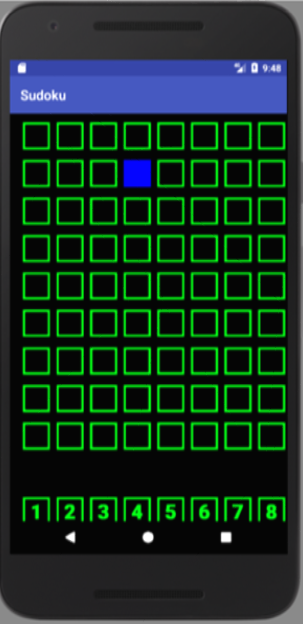
\includegraphics[width=4.5cm]{./Figure/alternative1.PNG}}\caption{Alternative 1}\label{Fig:alt1} \end{subfigure}
%
\hspace{1cm}
%
\begin{subfigure}[b]{4.5cm}\centering \frame{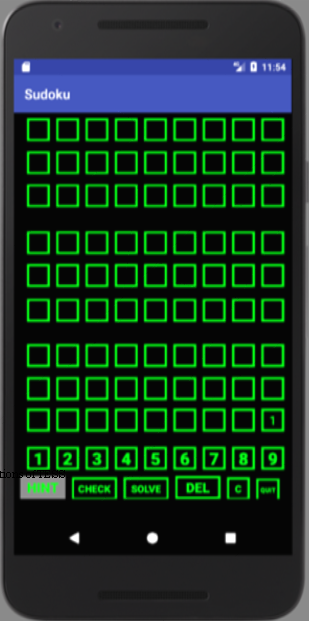
\includegraphics[width=4.5cm]{./Figure/alternative2.PNG}}\caption{Alternative 2} \label{Fig:alt2} \end{subfigure}\caption{Alternative Designs}\label{fig:altDesigns} \end{figure}


\section{System Implementation}
This section is about the overall system implementation of the TESS system. The activity diagram in Figure \ref{fig:activitydiagram} sets the overall overview of the implementation of the TESS system. Figure \ref{fig:sequencediagram} provides more details on the which system does specifically what. The two diagrams were the basis for the implementation part. Based on the 2 diagrams there would need to be at least 3 different user interfaces. 
\begin{wrapfigure}{r}{.3\textwidth}\begin{center} 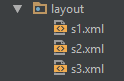
\includegraphics[width=1.0in]{./Figure/layout.PNG}\caption{Different UIs}\label{fig:UIs} \end{center}
\end{wrapfigure}
Figure \ref{fig:UIs} depicts the different UIs that are needed in the system. Layout s1 is the main page where the user can select the two option whether to solve or play a game. Figure \ref{fig:MainPage} depicts how the main page is seen by the user. When the user selects the play option that will direct them to the select difficulty page, shown in Figure \ref{fig:playPage}. From there they can either select one of the difficulties or they can select the continue option which will load the previous saved game. Once the select a difficulty, the game play page will display the board, as depicted in Figure \ref{fig:gamePlay}. If the user selects the solver option that will direct them to the game play screen; however, the complete board will be empty, as depicted in Figure \ref{fig:solverPage}.
\begin{figure*}[h]
	\centering
	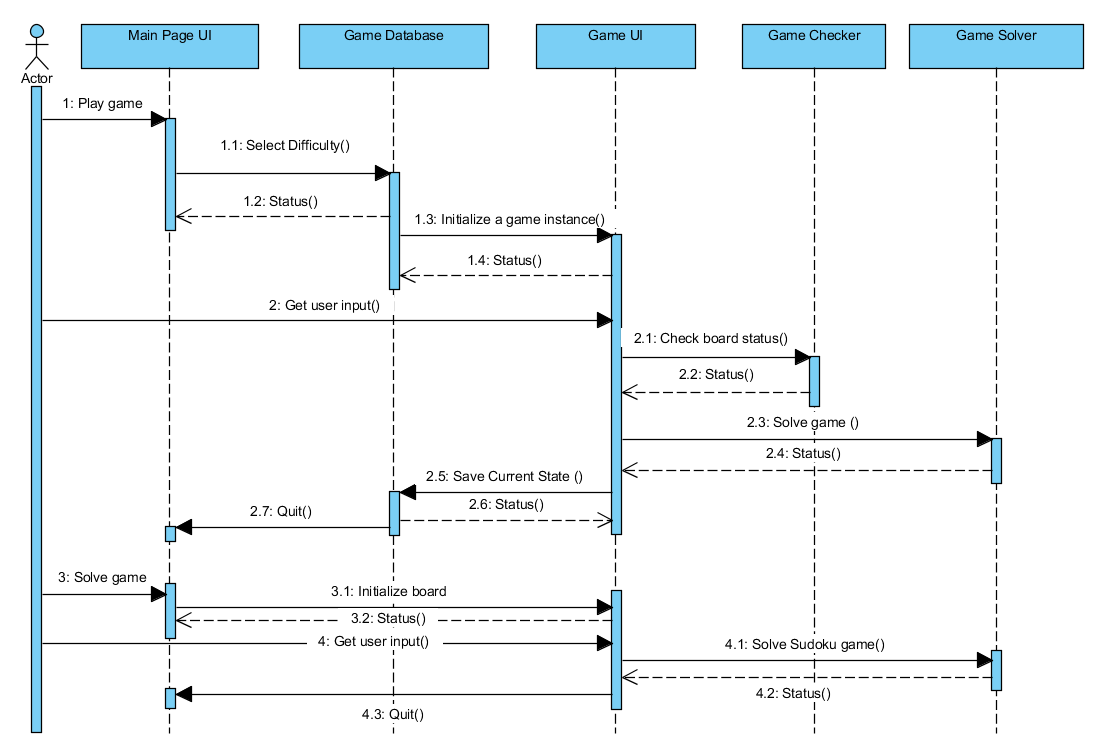
\includegraphics[width=5.0in]{./Figure/Sequence_Diagram.PNG}
	\caption{Sequence diagram of the TESS system.\cite{UMLDoc}}
	\label{fig:sequencediagram}
\end{figure*}


\begin{figure}[H]
\centering
\begin{minipage}{.5\textwidth} \centering 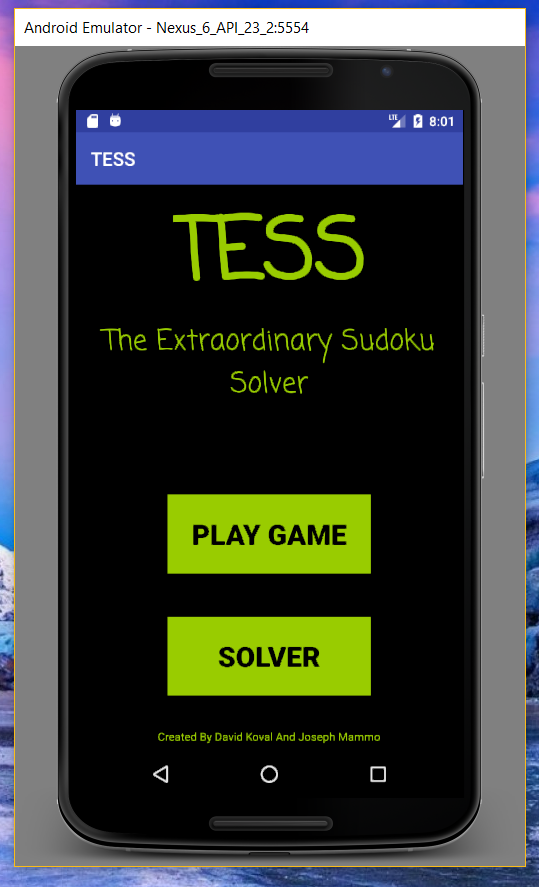
\includegraphics[width=2.0in]{./Figure/Main.PNG}\captionof{figure}{Main Page UI} \label{fig:MainPage}
\end{minipage}%
\begin{minipage}{.5\textwidth}\centering 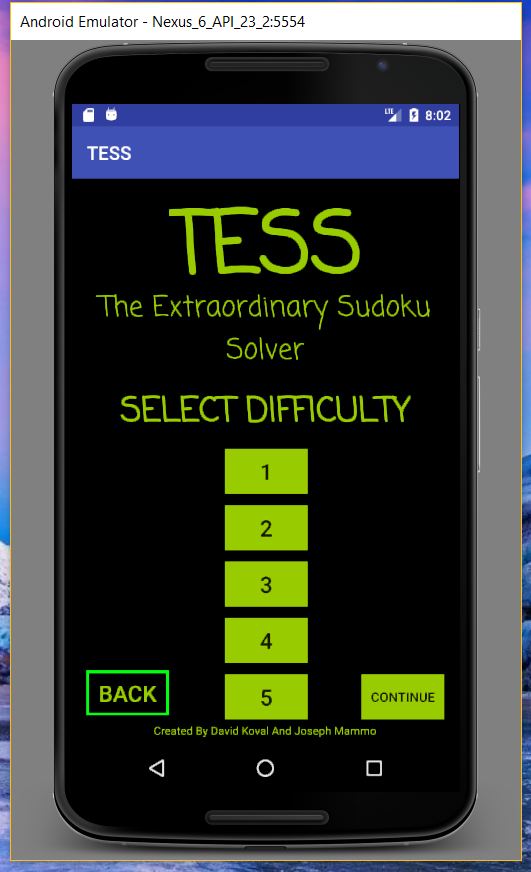
\includegraphics[width=2.0in]{./Figure/Play.PNG} \captionof{figure}{Play Option}\label{fig:playPage}
\end{minipage}%
\par\medskip\par\medskip
\begin{minipage}{.5\textwidth} \centering 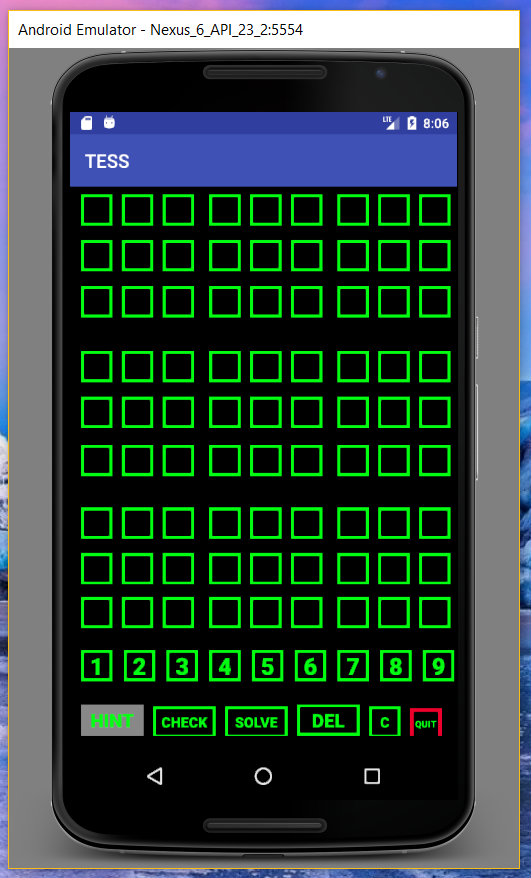
\includegraphics[width=2.0in]{./Figure/Solver.PNG}\captionof{figure}{Solver Option} \label{fig:solverPage}
\end{minipage}%
\begin{minipage}{.5\textwidth}\centering 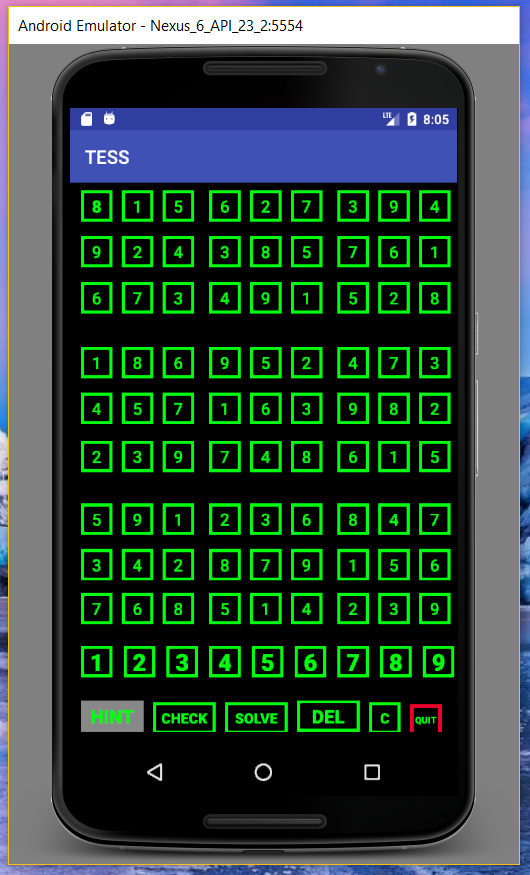
\includegraphics[width=2.0in]{./Figure/Solve.PNG} \captionof{figure}{Game Play}\label{fig:gamePlay}
\end{minipage}%
\end{figure}

Those previous figures depict the different UIs that are currently implemented. There are two main classes within the TESS system. One is the database class and the other one is the main class. The database builds the database on the users end and holds the different puzzles the app supports. The other class is the main class. There are a few different components to the main class, even though this class could have been broken up into smaller classes, due to the nature of the project, it all remained in the same class. Had the project been bigger, the class would have been separated into smaller classes. The main class houses the code creates the database class as well as inputs data into the database. It also contains the listeners to all the buttons. The reason the developers decided to leave every in one main class was because of all the listeners and at times some would need to be turned off and at other times, other would need to be. So everything was left in the main class to have easier access to all these listeners. There are also 2 other subclasses technically within the main page as well. There is the check class which checks the current board and if all the values are valid. Then there is the solver class, this is the bulk of the project. The subclass takes the current board and does a depth first search through the different possibilities to find the right one. This is only possible because of a pruning technique that is applied to the algorithm. 
\begin{figure*}[h]
	\centering
	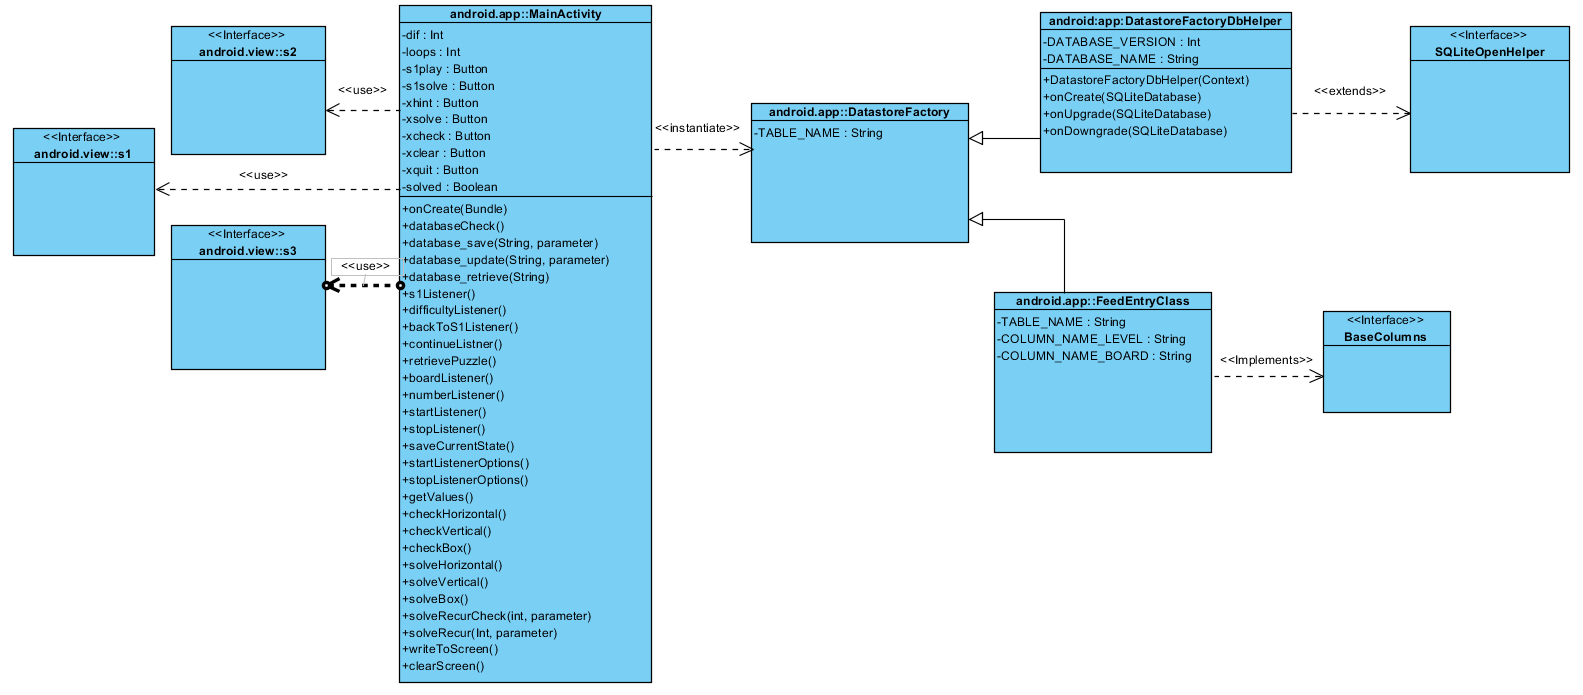
\includegraphics[width=5.0in]{./Figure/Class_Diagram.PNG}
	\caption{Class Diagram for TESS.}
	\label{fig:classdiagram}
\end{figure*}

The different classes in the TESS system are depicted in Figure \ref{fig:classdiagram}. The class diagram breaks the different class down and includes all the different variables and methods located in each class.

\section{System Testing}
This section will describe the testing plan for TESS and the different tests that will be conducted on it. This section will also display the results of the tests.

\subsection{Test Plan}
This section will describe the tesing plan for the system. Due to the nature of the project, the testing phase is only applicable to a small portion of the project. Since there is no input directly from the user and there are only buttons available for the user to use, the testing will be rather minimal. The project was created in such a way as to reduce the chance of errors, so the developers chose to use only buttons in the UI. There are a few major methods that do require testing, they are: solveHorizonal(), solveVertical(), solveBox(), and solveRecur(). For the first three methods there will be 2 tests each, one showing where it solves the expected square and the other where there is no way for it solve it. These cases are simple and are only used to solve the easy cases in the app in order to cut down the time of having the DFS run through the different possibilities. For the final method, solveRecur(), there will be 5 tests run, one from each difficulty to show that those puzzles can be solved and also 1 test case where the input is invalid. All of the aforementioned tests are unit tests, specifically Black-box tests. This specific type of test involves giving the program a set of input and testing it with the expected output. The other kind of unit tests are called White-box tests, in which there are multiple tests within a single unit test. For this project there is only one applicable place where White-box testing is necessary. In the solve function, solve(), that solves the entire puzzle, it relies on all four of the aforementioned methods as well as a secondary function that the solveRecur() calls on recursively, solveRecurCheck(). There will be 1 White-box test where each method is directly dependent on the other in order to produce the correct solution and also 1 other White-box test to perform the same test on invalid input. Due to the nature of the project, the integration testing is directly associated with the unit testing. The two different testing phases are intertwined within each other, so the aforementioned tests are also the integration tests as well. The integration tests are based on the bottom-up approach. There will be one specific system test that will be written because the only test that will need to be performed on the app is the performance test and this will tested by using one the most difficult Sudoku puzzles known to man. The test will check whether the app can solve it within the 5 second limit. There aren't any other system tests to create due to the nature of the app. These are all the tests that will need to be created and run to make sure the app works properly. Since this is still in the beta stages, there will be user testing and the app will be provided to select individuals to run the app and report back with their findings.

\subsection{Test Results}
This section will describe the test results in detail. The test results went as expected. As seen in Figure \ref{fig:tests}, all the tests passed. In Figure \ref{fig:horizontalTest} is an example of the many unit and integration tests that were written. The two different types of tests are interweaved so there aren't specific tests for one type. Most of these tests were written with the Black-box test design; however, the solve function was written with White-box test design in mind. These tests were created to make sure individual methods were working properly. Since the system is minimalistic and avoids any security risks there was only one main system test to design, this was the performance tests. As depicted in Figure \ref{fig:performanceTest}, the system test uses a time limit approach were it records the start time and the finish time. Then it converts the difference into seconds and returns whether the program solves it under the time constraint. This is one of the more important tests due the system constraints mentioned earlier. As shown per Figure \ref{fig:tests}, the performance test is under the time allotted for the program to solve any puzzle. The user tests are still in progress and there have not been any know issues yet. Overall, the tests were a success.
\begin{figure*}[ht]\centering
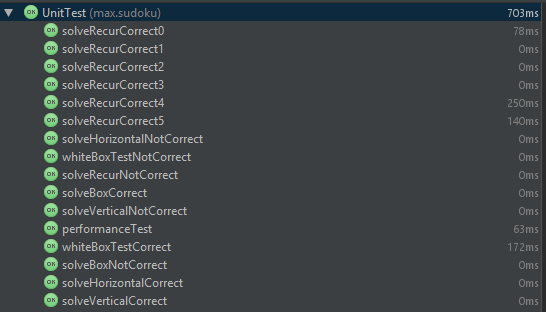
\includegraphics[width=4.0in]{./Figure/unit_test_results.PNG}
\caption{Results of test cases}\label{fig:tests}
\end{figure*}
\begin{figure*}[ht]\centering
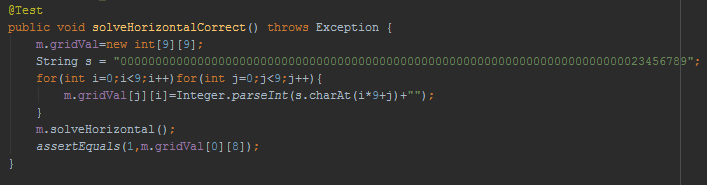
\includegraphics[width=4.0in]{./Figure/solve_horizontal_test.PNG}
\caption{Test: solveHorizontalTest()}\label{fig:horizontalTest}
\end{figure*}
\begin{figure*}[ht]\centering
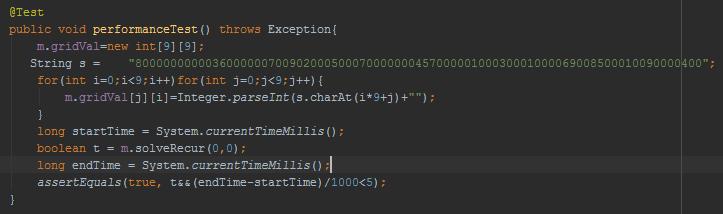
\includegraphics[width=4.0in]{./Figure/performance_test.PNG}
\caption{Test: performanceTest()}\label{fig:performanceTest}
\end{figure*}


\section{Conclusions} \todo{}
This is the conclusions section.

Overall summary of design methodologies, key creative approaches and potential
contribution/impact. \cite{BobCarpenter2013}
\cite{UMLDoc}

\bibliographystyle{IEEEtran}
\bibliography{Bibliography}

 
\end{document}